\documentclass[11pt,english,a4paper]{article}

\usepackage[utf8]{inputenc}          % Allows UTF-8 encoded characters in the .tex-file.
\usepackage{babel,csquotes,textcomp} % Set LaTeX to structure the content following international academic standards.
\usepackage[titletoc,toc]{appendix}
\usepackage{subfig}

\usepackage{hyperref}
\usepackage{graphicx}
\usepackage{pdfpages}
\usepackage{listings}
\usepackage{wrapfig}
\usepackage{color,colortbl}
\usepackage{lettrine}
\usepackage[font={small,it}]{caption}
\usepackage{multirow}
\usepackage{tabularx}
\usepackage{footnote}
\usepackage{enumitem}
\usepackage{amsmath}

\usepackage[
    backend=biber,
    style=numeric
]{biblatex}
\addbibresource{refs.bib}

\lstset{ %
  basicstyle=\ttfamily\small,     
  backgroundcolor=\color{white},   % choose the background color
  breaklines=true,                 % automatic line breaking only at whitespace
  captionpos=b,                    % sets the caption-position to bottom
  commentstyle=\color{mygreen},    % comment style
  escapeinside={\%*}{*)},          % if you want to add LaTeX within your code
  keywordstyle=\color{blue},       % keyword style
  stringstyle=\color{mymauve},     % string literal style
}

\title{Lab report \\ Frequency Counters}
\author{Aril Schultzen}

\begin{document}
\maketitle
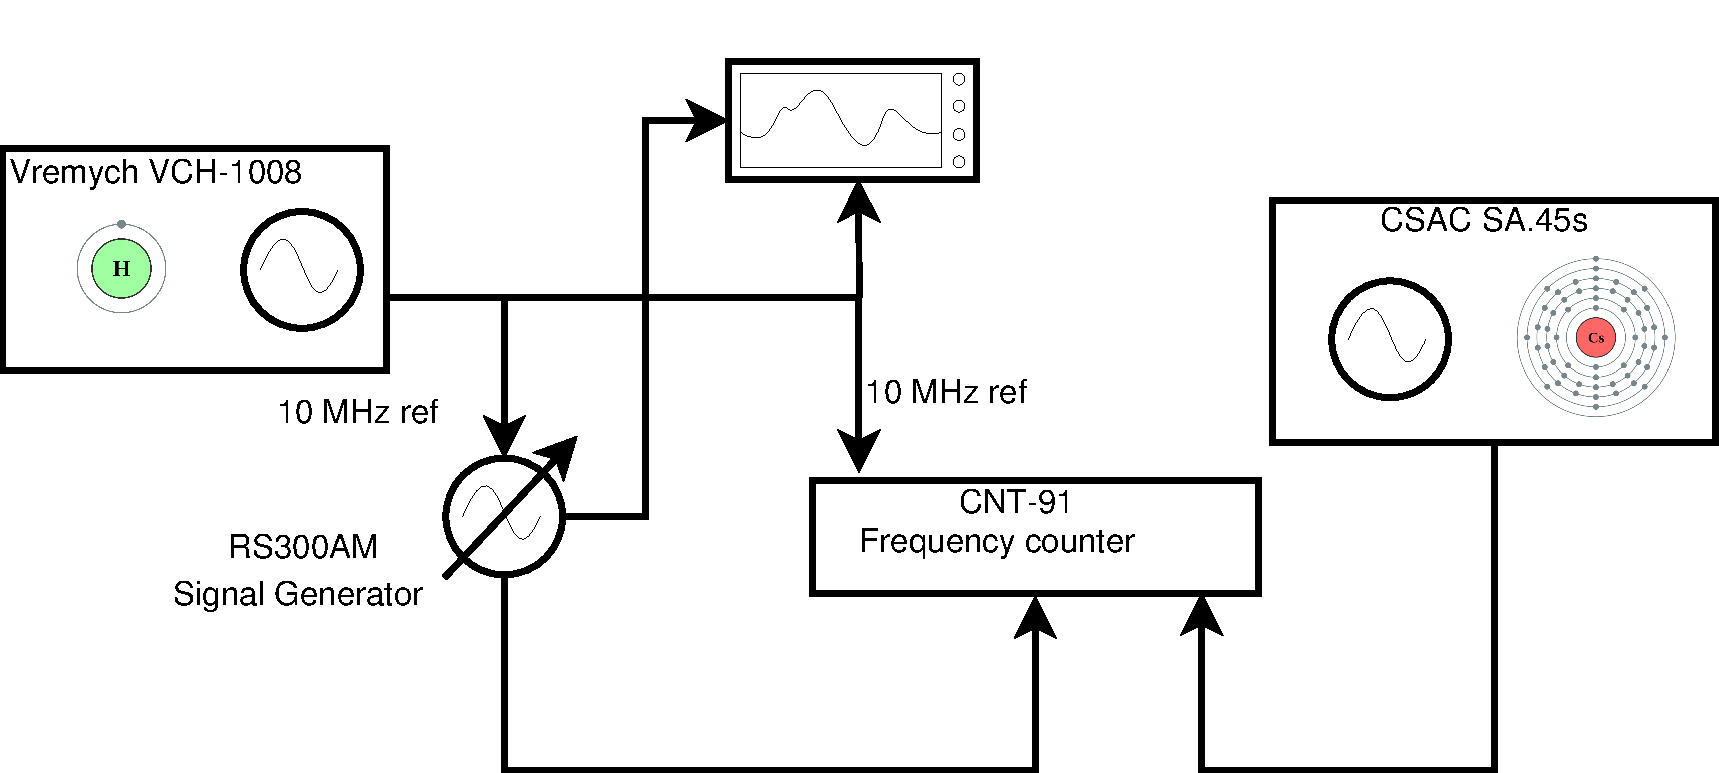
\includegraphics[width=1 \textwidth]{lab_report_diagram.pdf}
\section{Objective}
To gain an intuitive and visual understanding (of what?)

\section{Equipment}
\begin{itemize}
  \item Pendulum CNT-91, Frequency counter
  \item Rohde \& Scwarz 300AM, signal generator
  \item Tektronix MD0-4000-6 Oscilloscope
  \item Stopwatch, generic
  \item CSAC, oscillator to measure
  \item Passive Hydrogen maser, frequency reference
  \item RG-58 or RG223 cables
\end{itemize}

\section{Part A, frequency characterization}
\begin{figure}[!htb]
  \centering
  \subfloat[Oscilloscope capture 14:10:41]{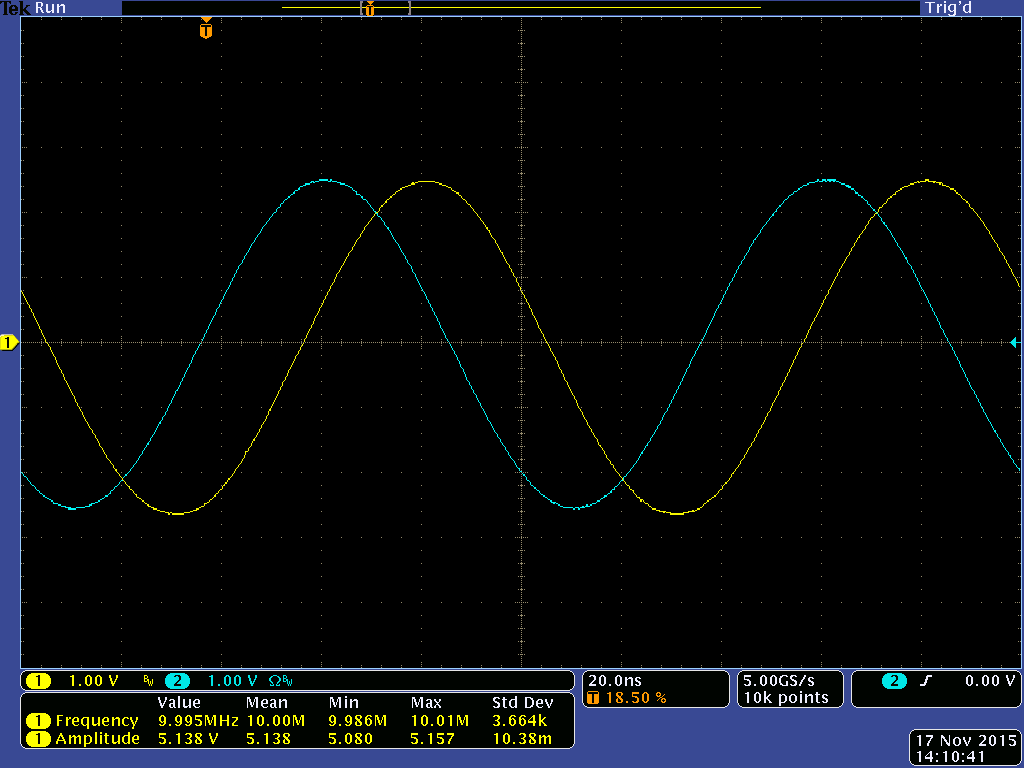
\includegraphics[width=0.5\textwidth]{del_A_kjapp_CSAC.png}\label{fig:f1}}
  \hfill
  \subfloat[Oscilloscope capture 14:10:48]{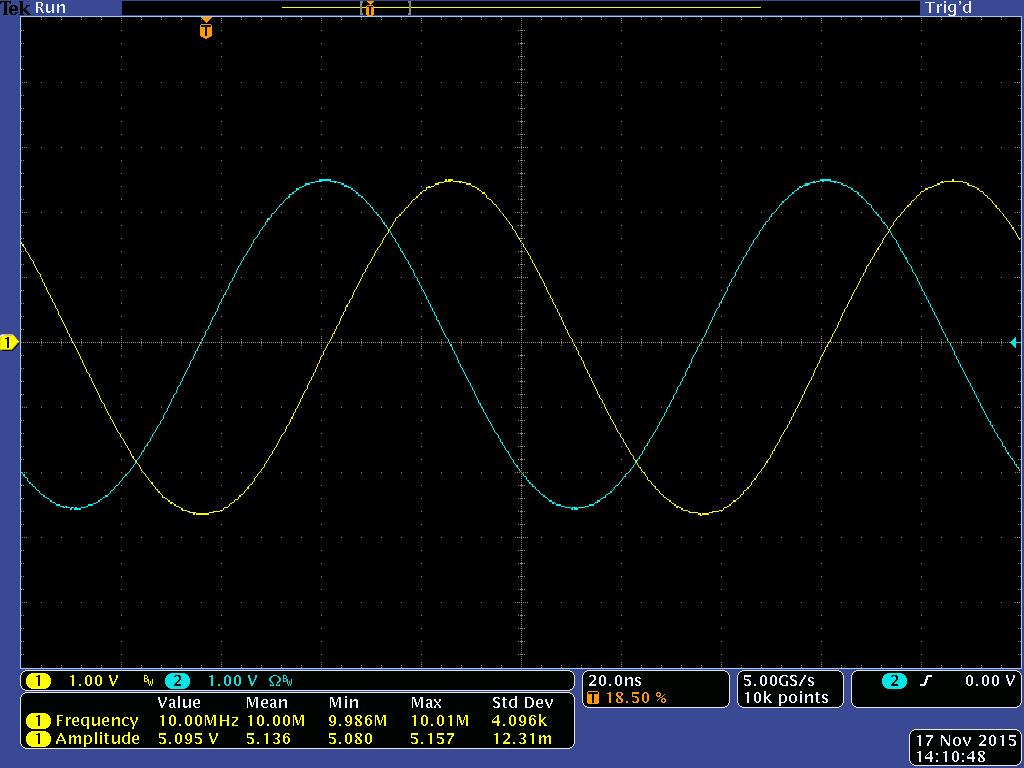
\includegraphics[width=0.5\textwidth]{del_A_kjapp_CSAC2.png}\label{fig:f2}}
  \caption{Oscilloscope captures}
\end{figure}
Figure \ref{fig:f1} and \ref{fig:f2} is two screen shots taken from the oscilloscope. The yellow line is the Passive hydrogen maser, the blue is the CSAC. The oscilloscope is triggering on the input from the CSAC. 

\subsection{Observations}
The two images shows the yellow line moving towards the right, indicating that the CSAC is a bit fast. When set to trigger on the maser instead, the effect is reversed, the blue line moves towards the left. 

\subsection{Measuring relative frequency error}
The period for each of the signals are 100 ns. By measuring the time it took for the two signals to go from being in phase once to twice (in phase, out of phase, in phase again), a relative frequency error can be calculated:

\begin{displaymath}
\frac{period}{phase-in-out-in} = \frac{100 ns}{160 s} = 0,625 ns/s
\end{displaymath}
\newline
It's worth noting that the phase-in-out-in time was measured using my wristwatch and that the accuracy of the measurement was anything but accurate. This is not a problem since the oscillators where measured with extremely high resolution.
The same principle applies to the oscilloscope concerning its lack of external frequency reference.   
\newpage

\section{Part 2: Frequency counting: Resolution and trigger noise: BTB}
The setup was reconfigured:
\begin{center}
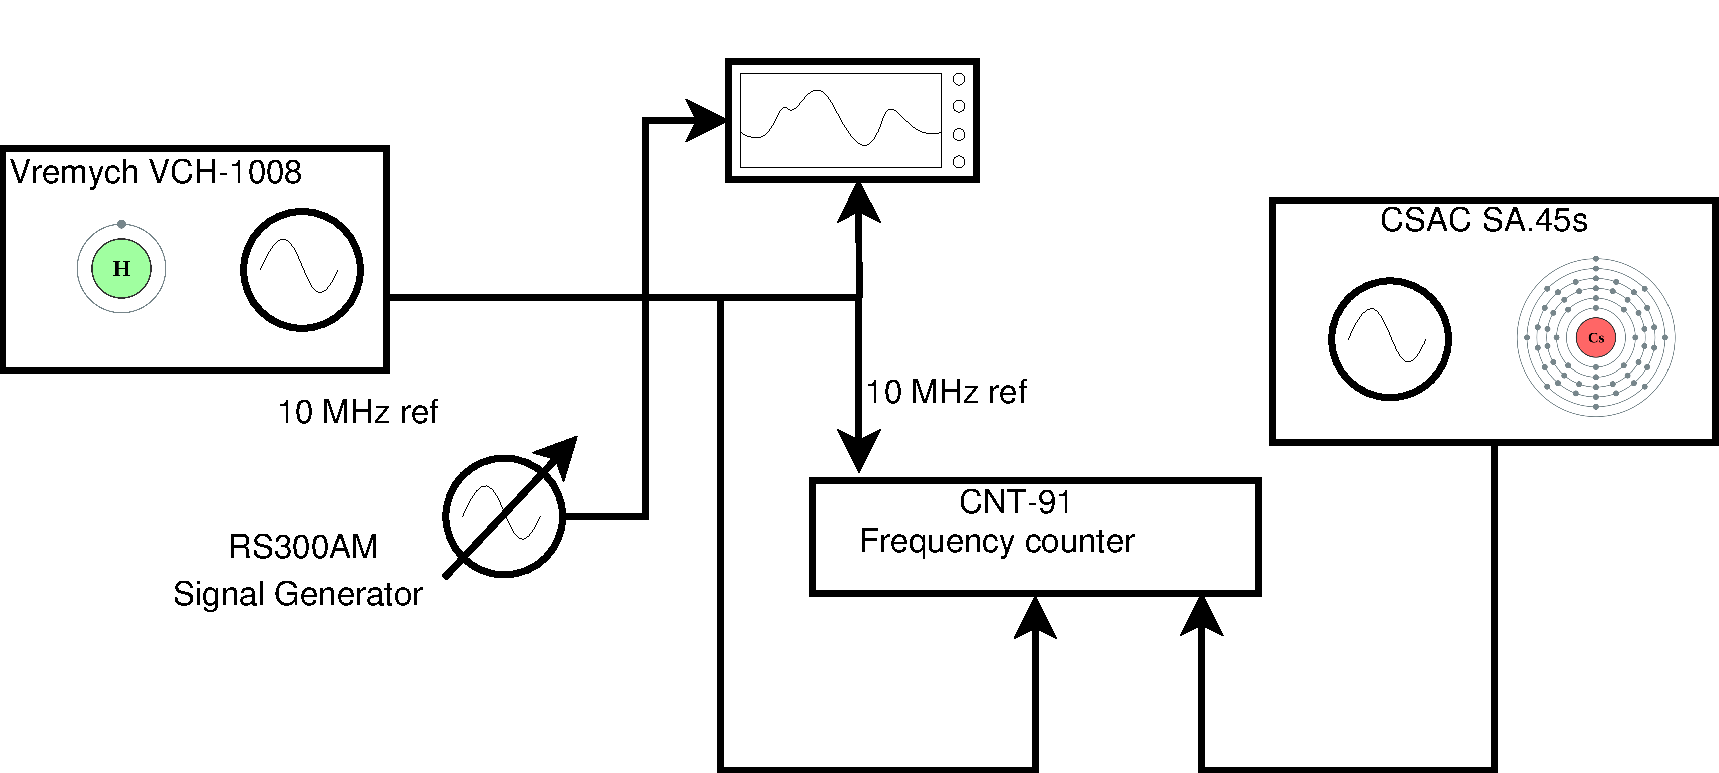
\includegraphics[width=1 \textwidth]{lab_report_diagram_del2.pdf}
\end{center}
The frequency counter now measures the maser (on input A) and uses it as reference. TimeView was then used to measure the frequency on input A, doing 200 samples with 1 s interval.

\subsection{Observations}
\subsubsection{Trigger resolution}
According to the User Manual for the CNT 9x Series, the resolution for Period A,B Back-to-Back is 50 ps rms. By observing the Alla deviation for the measurement (\ref{fig:allan_dev1}) the same can be observed.

\begin{figure}[!htb]
  \caption{Allan deviation for 200 samples at 1 s sample rate of 10MHz from the Passive Hydrogen maser.}
  \centering
    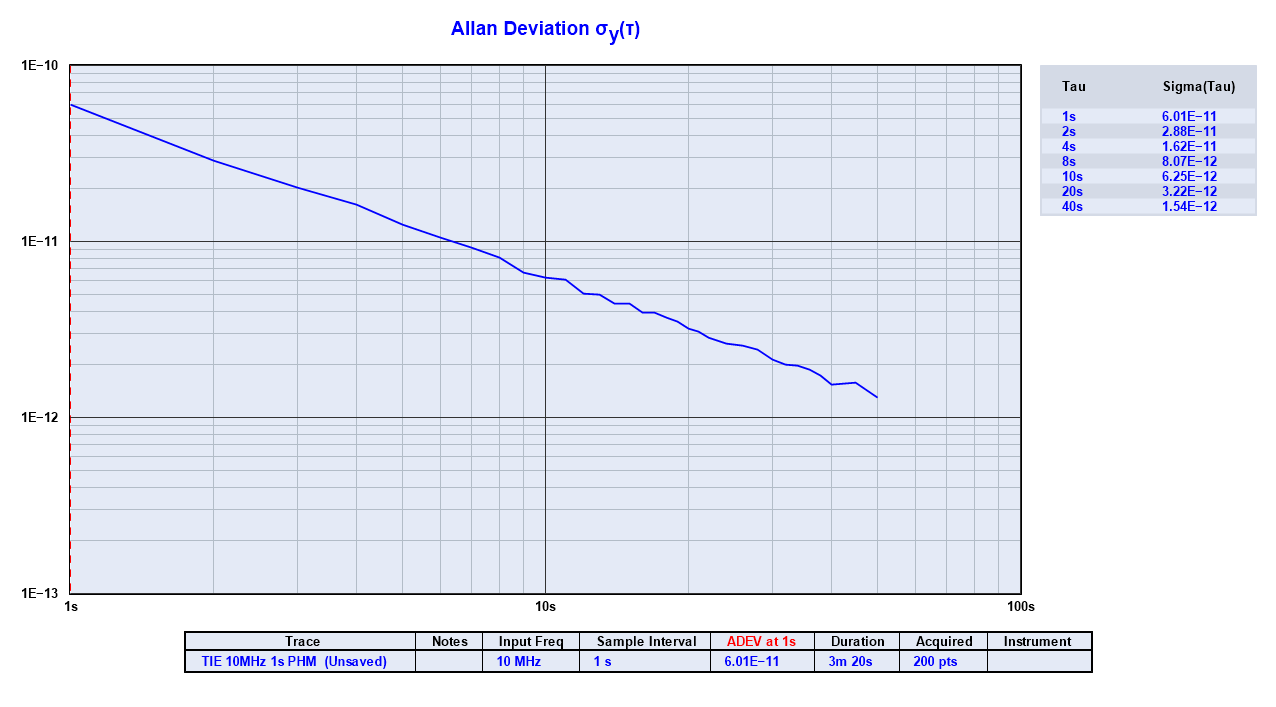
\includegraphics[width=1\textwidth]{phm10mhz1s_allan.png}
    \label{fig:allan_dev1}
\end{figure}
At the 1 second mark, the Allan Deviation is 8.23E-11 (around 82,3 ps) which seems about right considering start and stop at 50 ps (each) rms. 

\begin{figure}[!htb]
  \caption{Modified Allan deviation for 200 samples at 1 s sample rate of 10MHz from the Passive Hydrogen maser.}
  \centering
    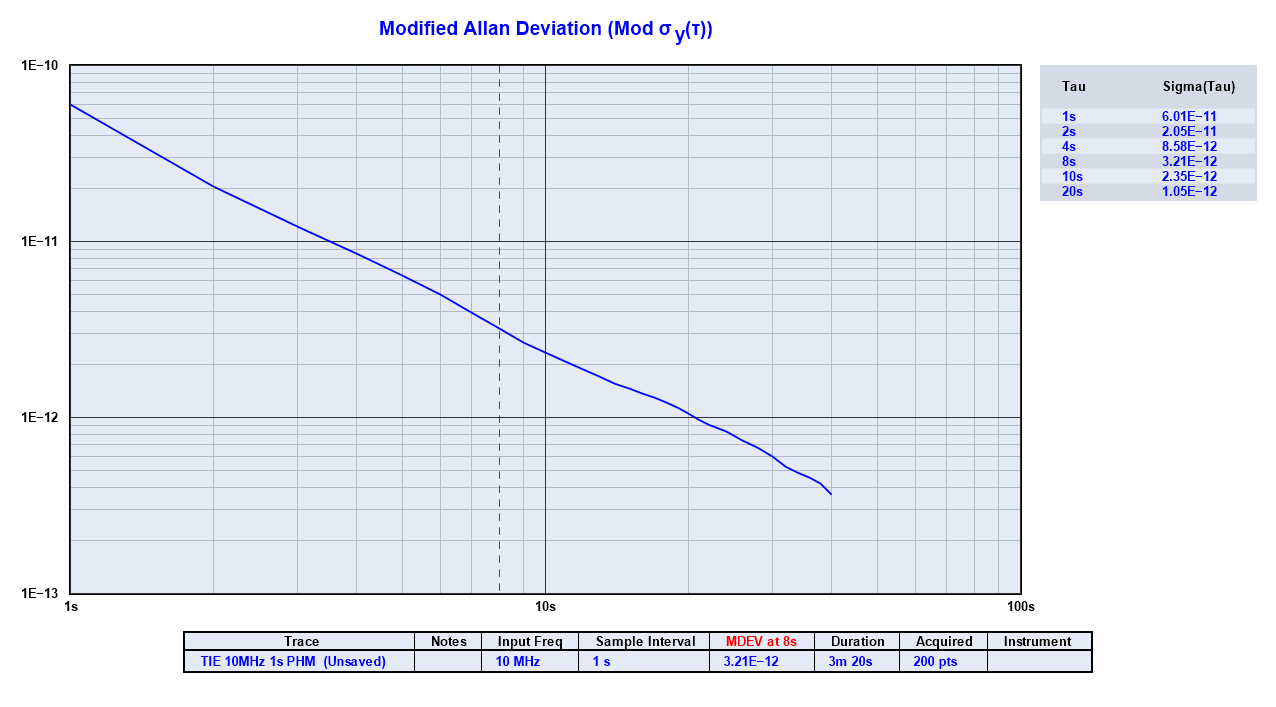
\includegraphics[width=1\textwidth]{phm10mhz1s_modified_allan.png}
    \label{fig:mod_allan_dev1}
\end{figure}
When observing the Modified Allan deviation for the same data (\ref{fig:mod_allan_dev1}), it becomes clear that the dominant type of noise is flicker noise (-1 slope).

\newpage
\subsubsection{Trigger level}
When raising the trigger level from 0 V to 1.2 V, more noise is introduced. This is because the slope of the signal is steeper at 0 V than at 1.2 V. The lower slope results in a less accurate trigging. 

\section{Part 2: Frequency counting: Resolution and trigger noise: TIE}


\end{document}                     